\documentclass[acmsmall, screen, dvipsnames]{acmart}
%% Suppress _everything_.
\pagestyle{plain}
\renewcommand\footnotetextcopyrightpermission[1]{}

%% \acmISBN{}
%% \acmDOI{}
\authorsaddresses{}
%% \setcopyright{none}
\settopmatter{printacmref=false,printccs=false,printfolios=false}
%% \acmPrice{}

\acmVolume{$\infty$}
\acmNumber{$\infty$}
\acmArticle{$\infty$}
\acmYear{$\infty$}
\acmMonth{0}


%% %% alternatively
%% \documentclass[dvipsnames]{article}
%% %% \usepackage[papersize={6.75in,8.75in},margin=1.5cm]{geometry}
%% %% \usepackage[papersize={6.75in,10in},margin=1.5cm]{geometry}
%% \usepackage[a5paper,margin=1cm]{geometry}
%% \usepackage{libertine}
%% \usepackage{euler} % the AMS Euler math font. Not compatible with acmart.cls.

\usepackage{amssymb,amsmath,amsthm,latexsym}
\usepackage{mathpartir}
\usepackage{multirow}
\usepackage{url,hyperref}
\usepackage{stmaryrd}           % for semantic brackets
\usepackage{mathtools}          % for \dblcolon
\usepackage{accents}            % for \underaccent
\usepackage{tikz,tikz-cd}       % Hasse & commutative diagrams.
\usepackage{adjustbox}          % aligning tikz diagrams vertically w/ tables.p


%% Commands
%% \newtheorem{theorem}{Theorem}
%% \newtheorem{definition}{Definition}
%% \newtheorem{corollary}{Corollary}
%% \newtheorem{conjecture}{Conjecture}
%% \newtheorem{lemma}{Lemma}
\newtheorem{principle}{Principle}

\newcommand{\todo}[1]{{\color{red}#1}}

\newcommand{\bnfeq}{\dblcolon=}
\newcommand{\defeq}{\overset{\ms{def}}{=}}

\newcommand{\ms}[1]{\ensuremath{\mathsf{#1}}}
\newcommand{\mb}[1]{\ensuremath{\mathbf{#1}}}
\newcommand{\mi}[1]{\ensuremath{\mathit{#1}}}
\newcommand{\mc}[1]{\ensuremath{\mathcal{#1}}}

\newcommand{\GG}{\Gamma}

\newcommand{\N}{\mathbb{N}}
\newcommand{\x}{\times}
\newcommand{\fn}{\lambda}
\newcommand{\binder}{.\,}
\newcommand{\bind}[1]{{#1}\binder}
\newcommand{\sub}[1]{\{{#1}\}}
\newcommand{\fix}{\ms{fix}}

%% TODO: get rid of \Disc, \Codisc.
\newcommand{\Disc}{{\color{red}\square}}
\newcommand{\Codisc}{{\color{red}\lozenge}}

\newcommand{\den}[1]{\llbracket{#1}\rrbracket}

%% Category & preorder theory
\newcommand{\id}{\ms{id}}
\newcommand{\op}{\ms{op}}
\newcommand{\iso}{\ms{core}}
\renewcommand{\path}{\ms{path}}

\newcommand{\isoto}{\simeq}
\newcommand{\pathto}{\sim}

%% tones: mono, anti, discrete, bivariant
\newcommand{\tm}{\id}                        % monotone / id
\newcommand{\ta}{{\color{ForestGreen}\op}}   % antitone / op
\newcommand{\ti}{{\color{NavyBlue}\iso}}     % invariant/ core
\newcommand{\tb}{{\color{Bittersweet}\path}} % bivariant/ path

\newcommand{\tc}{\cdot}         % tone composition

\newcommand{\h}[3]{#1 : {#2}^{#3}}
\newcommand{\hm}[2]{\h{#1}{#2}{\tm}}
\newcommand{\ha}[2]{\h{#1}{#2}{\ta}}
\newcommand{\hi}[2]{\h{#1}{#2}{\ti}}
\newcommand{\hb}[2]{\h{#1}{#2}{\tb}}

\newcommand{\mto}{\overset{\tm}{\to}}
\newcommand{\ato}{\overset{\ta}{\to}}
\newcommand{\ito}{\overset{\ti}{\to}}
\newcommand{\bto}{\overset{\tb}{\to}}


%% ---- Front matter ----
\title{Tones and Types}
%% alternate title: Tone theory
%% alternate title: Tonality inference
\author{Michael Arntzenius}
%% \email{daekharel@gmail.com}
\date{\todo{16 November 2017 -- ???}}


%% \setlength{\parskip}{0.4em}
%% \setlength{\parindent}{0em}


\begin{document}
\maketitle

\section{A preamble on preorders}

A preorder is a relation $a \le b$ satisfying:
\begin{enumerate}
\item \textbf{Reflexivity:} $a \le a$.
\item \textbf{Transitivity:} If $a \le b$ and $b \le c$ then $a \le c$.
\end{enumerate}

A good example of a preorder is ``lists under containment'', where $a \le b$ iff
every element of $a$ is also in $b$.

Preorders are partial orders, sans antisymmetry. Let $a \equiv b$ iff $a \le b$
and $b \le a$. Antisymmetry means $a \equiv b$ implies $a = b$. However, under
list containment, $[0,1] \equiv [1,0]$, but $[0,1] \ne [1,0]$.

To a category theorist, a preorder is a ``thin'' category, where between any two
objects there is at most one morphism. I suspect much of the ``tone theory'' in
this document, ostensibly about maps between preorders, extends to functors
between categories.


\subsection{Tones (categorically)}

\todo{TODO: this note is useful, but should go somewhere else}

\newcommand{\elemset}[1]{\ensuremath{\mc{U}({#1})}}
\newcommand{\elemsetfn}[0]{\mc{U}}
\renewcommand{\elemset}[1]{\ensuremath{|{#1}|}}
\renewcommand{\elemsetfn}[0]{\elemset{-}}

Let $\elemsetfn{} : \mb{Preorder} \to \mb{Set}$ be the forgetful functor which
takes a preorder to its set of elements.

\begin{definition}
  A tone $s$ is a functor $-^s : \mb{Preorder} \to \mb{Preorder}$ such that
  $\elemset{-^s} = \elemsetfn$.
\end{definition}

In particular, for any preorder $A$ and monotone map $f$,
\begin{enumerate}
\item $|A^s| = |A|$, i.e. a tone functor transforms only the \emph{ordering},
  not the elements, of a preorder.
\item $|f^s| = |f|$, i.e. a tone functor does not change the behavior of
  functions.
\end{enumerate}

A more ``categorical'' definition might require only a natural isomorphism
$\iota : \elemsetfn \isoto \elemset{-^s}$. I'm not comfortable generalizing that
far yet.
%
It's also unclear how to generalize this definition to tones of functors on
\mb{Cat}.


\section{Tones}

\begin{center}
  \begin{tabular}{clc@{\hskip 0.25em}c@{\hskip 0.25em}c}
    \multicolumn{1}{c}{\textbf{Tone}}
    & \multicolumn{1}{c}{\textbf{Name}}
    %% & \multicolumn{1}{c}{\textbf{Respects}}
    & \multicolumn{3}{c}{\textbf{Property of $f$}}
    \\\hline
    \tm & \text{Monotone}
    %% & \text{ordering}
    & $x \le y$ &$\implies$& $f(x) \le f(y)$
    \\
    \ta & \text{Antitone}
    %% & \text{opposite ordering}
    & $x \ge y$ &$\implies$& $f(x) \le f(y)$
    \\
    \tb & \text{Bivariant}
    %% & \text{equivalence closure or ``paths''}
    & $x \le y \vee y \le x$ &$\implies$& $f(x) \le f(y)$
    \\
    \ti & \text{Invariant}
    %% & \text{induced equivalence or ``isomorphisms''}
    & $x \le y \wedge y \le x$ &$\implies$& $f(x) \le f(y)$
  \end{tabular}
\end{center}

Tones are ways a function $f$ may respect a preordering. I will consider four
tones: \tm, \ta, \tb, and \ti.

\begin{enumerate}
\item $\tm$ is monotone (order-preserving).
\item $\ta$ is antitone (order-inverting).
\item $\tb$ is bivariant: both monotone and antitone.
\item $\ti$ is invariant, respecting only equivalence.
\end{enumerate}

%% In posets, antisymmetry trivializes invariance (because $x \le y \wedge y \le x
%% \implies x = y \implies f(x) = f(y)$), so we sometimes call $\ti$ the
%% ``discrete'' tone, because it respects only the discrete ordering.


\subsection{Tones transform orders}

Consider preorders $A, B$. Let $A^\op$ be $A$, ordered oppositely. Now, observe
that

\begin{center}
  $f : A \to B$ is antitone

  \nopagebreak
  \emph{iff}
  \nopagebreak

  $f : A^\op \to B$ is monotone
\end{center}

So ``antitone'' is a special case of ``monotone''! This observation generalizes:
every tone is really monotonicity with a transformation applied to the domain's
ordering. So \textbf{tones transform orders.}
%
I write $A^s$ for the preorder $A$ transformed by the tone $s$, defined as
follows:

\begin{center}
  \begin{tabular}{clc@{\hskip 0.25em}c@{\hskip 0.25em}l}
    {\textbf{Tone}}
    & {\textbf{Meaning}}
    & \multicolumn{3}{c}{\textbf{Transformation on $A$}}
    \\\hline
    \tm & \text{same ordering}
    & $a \le b : A$ &$\iff$& $a \le b : A^\tm$
    \\
    \ta
    & \text{opposite ordering}
    & $a \ge b : A$ &$\iff$& $a \le b : A^\op$
    \\
    \tb{}
    & \text{equivalence closure}
    & $a \le b \vee b \le a : A$ &$\ \implies$& $a \le b : A^\path$
    \quad \emph{\small (see \ref{sec:defining-path})}
    \\
    \ti
    & \text{induced equivalence}
    & $a \le b \wedge b \le a : A$ &$\iff$& $a \le b : A^\iso$
  \end{tabular}
\end{center}

With this, we can state the theorem generalizing our observation:
\begin{theorem}[Tones transform orders]\label{thm:tones-transform-orders}
  %% Given a function $f : A \to B$ between preorders $A$, $B$:
  ~
  \begin{center}
    $f : A \to B$ has tone $s$\\
    iff\\
    $f : A^s \to B$ is monotone
  \end{center}
\end{theorem}

%% \begin{proof} Exercise for the reader. \end{proof}

From this point on, when I write $f : A \to B$, I mean implicitly that $f$ is
monotone; and therefore $f : A^s \to B$ means that $f$ has tone $s$.
%
Also, there is one more property of tones we will need:

\begin{theorem}[Functoriality of tones]\label{thm:tone-functoriality}
  If $f : A \to B$ then $f : A^s \to B^s$.
  %% \[\text{If}~ f : A \to B ~\text{then}~ f : A^s \to B^s\text{.}\]
\end{theorem}
%% \begin{proof} Exercise for the reader. \end{proof}

Together, these theorems define a more general notion of tone: a tone $s$ is a
transformation $-^s$ on the ordering component of a preorder (i.e. $A^s$ must
have the same elements as $A$) satisfying Theorem \ref{thm:tone-functoriality},
whose interpretation as a property of functions is given by Theorem
\ref{thm:tones-transform-orders}.

\subsection{On defining \ms{path} directly} \label{sec:defining-path}

$A^\path$ is the smallest preorder satisfying
\[ a \le b \vee b \le a : A \implies a \le b : A^\path \]

Unfortunately, $A^\path$ is not so easy to define \emph{directly}, without
language like ``the smallest preorder satisfying''.
%
In particular, the reverse implication, from $a \le b : A^\path$ to $a \le b
\vee b \le a : A$, does not always hold. A good counterexample is the
\ms{fencepost} ordering on the naturals, where $a \le a+1$ for even $a$, and $a
\ge a+1$ for odd $a$:

\todo{TODO: Diagram}.

Note that $a \le b \vee b \le a : \ms{fencepost} \iff |a-b| \le 1$, which isn't
transitive! Instead, $\ms{fencepost}^\path$ is the \emph{transitive closure} of
$|a - b| \le 1$, which makes everything equivalent:
\[ 0 \equiv 1 \equiv 2 \equiv 3 \equiv 4 \equiv ... \]

However, a direct definition of $A^\path$ is possible, using \emph{paths}:
``zig-zagging'' lists $a_0, a_1, ..., a_n$ such that $a_i \le a_{i+1} \vee a_i
\ge a_{i+1} : A$. Then $a \le b : A^\path$ iff there is a path starting from $a$
and ending at $b$.


\subsection{Tone operators}

\begin{figure*}
  \begin{mathpar}
    %% "baseline=(current bounding box.center)" incantation taken from
    %% https://tex.stackexchange.com/questions/220531/how-to-align-tikzpicture-and-text-in-a-table/220543#220543
    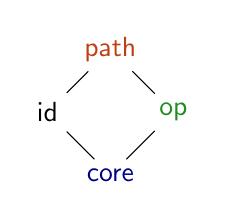
\begin{tikzpicture}[scale=0.8,baseline=(current bounding box.center)]
      \node (top)  at ( 0, 1) {$\tb$};
      \node (bot)  at ( 0,-1) {$\ti$};
      \node (-1)   at (-1, 0) {$\tm$};
      \node (1)    at ( 1, 0) {$\ta$};
      \draw (top) -- (-1) -- (bot) -- (1) -- (top);
    \end{tikzpicture}

    %% \begin{array}{cc|rrrrr}
    %%   \multicolumn{2}{c|}{\multirow{2}{*}{$s \wedge t$}}
    %%   & \multicolumn{4}{c}{t}\\
    %%   && \tm & \tb & \ta & \ti\\\hline
    %%   \multirow{4}{*}{$s$}
    %%   & \tm & \tm & \tm & \ti & \ti\\
    %%   & \tb & \tm & \tb & \ta & \ti\\
    %%   & \ta & \ti & \ta & \ta & \ti\\
    %%   & \ti & \ti & \ti & \ti & \ti
    %% \end{array}
    \begin{array}{c|rrrrr}
      s \wedge t & \tm & \tb & \ta & \ti\\\hline
      \tm & \tm & \tm & \ti & \ti\\
      \tb & \tm & \tb & \ta & \ti\\
      \ta & \ti & \ta & \ta & \ti\\
      \ti & \ti & \ti & \ti & \ti
    \end{array}

    \begin{array}{cc|rrrr}
      \multicolumn{2}{c|}{\multirow{2}{*}{$s \tc t$}}
      & \multicolumn{4}{c}{t}\\
      && \tm & \ta & \ti & \tb\\\hline
      \multirow{4}{*}{$s$}
      & \tm & \tm & \ta & \ti & \tb\\
      & \ta & \ta & \tm & \ti & \tb\\
      & \ti & \ti & \ti & \ti & \ti\\
      & \tb & \tb & \tb & \tb & \tb
    \end{array}
  \end{mathpar}
  \caption{Tone lattice, meet, and composition}
  \label{fig:tone-ops}
\end{figure*}

Figure~\ref{fig:tone-ops} defines two operators on tones:
\begin{enumerate}
\item Meet $s \wedge t$ is greatest lower bound in the lattice ordered $\ti <
  \{\tm, \ta\} < \tb$. This gives the general tone of the pairing $\langle f,
  g\rangle : A^{s \wedge t} \to B \times C$ of two functions $f : A^s \to B$ and
  $g : A^{t} \to C$.

  \todo{TODO: isn't this just intersection of the relations? if $R(a,b)$ and
    $S(a,b)$ are preorders, is $R(a,b) \wedge S(a,b)$ reflexive and transitive?
    Yes (even though $R(a,b) \vee S(a,b)$ isn't always)! So then $x \le y : A^{s
      \wedge t} \iff x \le y : A^s \wedge x \le y : A^t$?}

\item Composition $s \tc t$ gives the tone of a composed function $g \circ f :
  A^{s\tc t} \to C$ when $f : A^s \to B$ and $g : B^t \to C$. Equivalently,
  $A^{s\tc t} = (A^s)^t$ for any preorder $A$.

  \todo{TODO: Likewise, this is just observing that tones compose to tones,
    right? But does this semantic operation match up with our syntactic
    definition of $s \tc t$?}
\end{enumerate}



Together, $\wedge$ and $\tc$ form a semiring, with the following panoply of
laws:\footnote{\todo{TODO: Reference ``I Got Plenty o' Nuttin'{}'' --- another
    use of variable annotations drawn from a semiring, and with similar (the
    same?) behavior of those annotations in the inference rules.}}

\begin{mathpar}
  \begin{array}{lr@{\hskip 0.5em}c@{\hskip 0.5em}l}
    \multicolumn{4}{c}{\textbf{Properties of } \wedge}
    \vspace{0.1em}\\
    \textbf{Associativity} & (s \wedge t) \wedge u &=& s \wedge (t \wedge u)\\
    \textbf{Commutativity} & s \wedge t &=& t \wedge s\\
    \textbf{Idempotence} & s \wedge s &=& s\\
    \tb~\textbf{is identity} & \tb \wedge s &=& s\\
    \ti~\textbf{absorbs} & \ti \wedge s &=& \ti\\
  \end{array}

  \begin{array}{lr@{\hskip 0.5em}c@{\hskip 0.5em}l}
    \multicolumn{4}{c}{\textbf{Properties of } \tc}
    \vspace{0.1em}\\
    \textbf{Associativity} & (s \tc t) \tc u &=& s \tc (t \tc u)\\
    \textbf{Identity} & \multicolumn{3}{c}{\tm \tc s = s = s \tc \tm}\\
    \tb~ \textbf{left-absorbs} & \tb \tc s &=& \tb\\
    \ti~ \textbf{left-absorbs} & \ti \tc s &=& \ti\\
    \ta~ \textbf{self-inverts} & \ta \tc \ta &=& \tm\\
  \end{array}

  \begin{array}{lr@{\hskip 0.5em}c@{\hskip 0.5em}l}
    \textbf{Left-distribution} & s \tc (t \wedge u) &=& (s \tc t) \wedge (s \tc u)\\
    \textbf{Right-distribution} & (s \wedge t) \tc u &=& (s \tc u) \wedge (t \tc u)
  \end{array}
\end{mathpar}

\todo{TODO: check the distribution laws hold!}


\subsection{Relation to Monotonicity Types}
\href{https://infoscience.epfl.ch/record/231867/files/monotonicity-types.pdf}{\emph{Monotonicity
    Types}} by Clancy, Miller, and Meiklejohn has similar tables for their
composition $\circ$ and ``contraction'' $+$ operators! However, instead of
bivariance they have constancy, a stricter condition.
%
Constancy corresponds to respecting the \emph{indiscrete ordering} (which sets
$a \le b$ for all $a,b$).\footnote{Indiscreteness (and its dual, discreteness)
  are also tones --- that is, functorial transformations on the ordering
  component of a preorder --- but they complicate things and are unused in
  Datafun, so I omit them. It is worth noting that discreteness and $\ti$
  coincide when restricted to posets, so many intuitions transfer from one to
  the other.}
%
Interestingly, because constancy is so much stricter than bivariance, their
composition operator is commutative.

They write $\uparrow$ for $\tm$, $\downarrow$ for $\ta$, $?$ for $\ti$, and
$\sim$ for constancy. They also add $=$ for the ``tone'' that \emph{only the
  identity function} has. This doesn't fit my framework; it cannot be phrased as
a transformation on orderings. However, it seems related to subtyping.


\section{A tonal sequent calculus}

These rules sent to me by Jason Reed. $T_s$ is the connective to internalizing
$-^s$.
\begin{mathpar}
  (A_1^{t_1}, ..., A_n^{t_n})^u = (A_1^{t_1 \tc u}, ..., A_n^{t_n \tc u})\\

  \infer[$T$-Right]{\GG \vdash A}{\GG^t \vdash T_t A}

  \infer[$T$-Left]{\GG{},A^{t\tc u} \vdash C}{\GG{}, (T_t A)^u \vdash C}

  \infer[Weakening]{\GG{}, A^t \vdash C \\ u \le t}{\GG{}, A^u \vdash C}

  \infer[Contraction]{\GG{},A^t, A^u \vdash C}{\GG{}, A^{t \wedge u} \vdash C}

  \infer[Cut]{\GG \vdash A \\ \Delta,A^t \vdash C}{\GG^t,\Delta \vdash C}
\end{mathpar}

I aim to adapt this into a natural-deduction-style system with proof terms,
i.e.\! a simply typed $\lambda$-calculus.

\todo{TODO: Revisit this. Think about what $T$-Left means, and Kevin Clancy's
  phrasing of the eliminator for his type as requiring tones compose to
  something $\le \tm$.}


\section{A bidirectional $\lambda$-calculus with tone inference}

\newcommand{\isfn}[4]{{#2}^{#1}\sqsubset {#3} \Rightarrow {#4}}
\newcommand{\subtype}[3]{{#2}^{#1}\sqsubset {#3}}
\newcommand{\converts}[3]{{#2}^{#1} \prec {#3}}

\newcommand{\infers}[3]{{#1} \Rightarrow {#2} \vdash {#3}}
\newcommand{\checks}[3]{{#1} \Leftarrow {#2} \vdash {#3}}

\begin{mathpar}
  \begin{array}{cccl}
    \text{tones} & s,t,u & \bnfeq & \tm ~|~ \ta ~|~ \tb ~|~ \ti
    \vspace{0.5em}\\
    \text{types} & A,B,C
    &\bnfeq& \ms{base} ~|~ A \to B ~|~ A \x B ~|~ \Box A ~|~ \op\;A
    \vspace{0.5em}\\
    \text{checking terms} & M
    &\bnfeq& N ~|~ \fn\bind{x} M ~|~ (M, M)
    ~|~ \mb{let}~x = N~\mb{in}~ M
    \vspace{0.5em}\\
    \text{inferring terms} & N
    &\bnfeq& M : A ~|~ x ~|~ N\;M ~|~ \pi_i\;N
    \vspace{0.5em}\\
    \text{contexts}
    & \GG &\bnfeq& \cdot ~|~ \GG{}, \h{x}{A}{s}
    \vspace{0.5em}\\
    \text{judgments}
    & J &\bnfeq&
    \checks{M}{\GG}{A}
    \\&&|& \infers{N}{\GG}{A}
    \\&&|& \subtype{s}{A}{B} ~|~ \converts{s}{A}{B}
  \end{array}
\end{mathpar}

\todo{TODO: explain my various abuses of notation, e.g. $\GG^t$ and $\GG_1
  \wedge \GG_2$}


\subsection{Typing rules}

\begin{mathpar}
  \infer{ }{\infers{x}{\h{x}{A}{\tm}}{A}}

  \infer{\checks{M}{\GG}{A}}{\infers{M : A}{\GG}{A}}

  \infer{\infers{N}{\GG}{A} \\ \subtype{t}{A}{B}}
        {\checks{N}{\GG^t}{B}}

  %% type-driven subtyping for checking
  \infer{\checks{M}{\GG}{A}}
        {\checks{M}{\GG^\ti}{\Box A}}

  \infer{\checks{M}{\GG}{A}}
        {\checks{M}{\GG^\ta}{\op\; A}}

  %% let-binding
  \infer{\infers{N}{\GG_1}{A} \\ \checks{M}{\GG_2,\, \h{x}{A}{s}}{C}}
        {\checks{\mb{let}~x = N~\mb{in}~M}{\GG_1{}^s \wedge \GG_2}{C}}

  %% introductions
  \infer{\checks{M}{\GG{},\, \h{x}{A}{s}}{B} \\ \tm \le s}
        {\checks{\fn\bind{x} M}{\GG}{A \to B}}

  \infer{\checks{M_1}{\GG_1}{A_1} \\ \checks{M_2}{\GG_2}{A_2}}
        {\checks{(M_1,M_2)}{\GG_1 \wedge \GG_2}{A_1 \x A_2}}

  %% eliminations
  \infer{\infers{N}{\GG_1}{A}
         \\ \converts{u}{A}{B \to C}
         \\ \checks{M}{\GG_2}{B}}
        {\infers{N\; M}{\GG_1{}^u \wedge \GG_2}{C}}

  \infer{\infers{N}{\GG}{A} \\ \converts{s}{A}{B_1 \x B_2}}
        {\infers{\pi_i\;N}{\GG^s}{B_i}}
\end{mathpar}


\subsection{Subtyping}
In $\subtype{s}{A}{B}$, the types $A$ and $B$ are inputs, and the tone $s$ is
output.

\begin{mathpar}
  \infer{ }{\subtype{\tm}{A}{A}}

  \infer{A~\ms{equiv}}{\subtype{\ti}{A}{A}}

  \infer{\subtype{s}{A}{B}}
        {\subtype{s \tc \ti}{A}{\Box B}}

  \infer{\subtype{s}{A}{B}}
        {\subtype{\tb \tc s}{\Box A}{B}}

  \infer{\subtype{s}{A}{B}}
        {\subtype{\ta \tc s}{(\op\; A)}{B}}

  \infer{\subtype{s}{A}{B}}
        {\subtype{s \tc \ta}{A}{\op\; B}}

  \infer{\subtype{s}{A_1}{A_2} \\ \subtype{t}{B_1}{B_2}}
        {\subtype{s \wedge t}{(A_1 \x B_1)}{A_2 \x B_2}}

  %% The function rules!
  \infer{\subtype{s}{A_1}{A_2} \\ \subtype{\tm}{B_1}{B_2} \\ \tm \le s}
        {\subtype{\tm}{(A_1 \to B_1)}{A_2 \to B_2}}

  \infer{\subtype{s}{A_1}{A_2} \\ \subtype{\ta}{B_1}{B_2} \\ \ta \le s}
        {\subtype{\ta}{(A_1 \to B_1)}{A_2 \to B_2}}

  \infer{\subtype{s}{A_1}{A_2} \\ \subtype{\tb}{B_1}{B_2} \\ \ti < s}
        {\subtype{\tb}{(A_1 \to B_1)}{A_2 \to B_2}}

  \infer{\subtype{\tb}{A_1}{A_2} \\ \subtype{\ti}{B_1}{B_2}}
        {\subtype{\ti}{(A_1 \to B_1)}{A_2 \to B_2}}
\end{mathpar}

\todo{Can these $t \le s$ constraints be turned into ``composing with $u$ is
  $\ge \tm$'', for some choice of $u$ depending on $t$?}


\subsection{Spine subtyping}

In $\converts{s}{A}{B}$, the type $A$ is input, the \emph{shape} of $B$ (either
$- \to -$ or $- \x -$) is input, the actual types in $B$ are outputs, and the
tone $s$ is output.
\begin{mathpar}
  \infer{ }{\converts{\tm}{A}{A}}

  \infer{\converts{s}{A}{B}}{\converts{\tb\tc s}{\Box A}{B}}

  \infer{\converts{s}{A}{B}}{\converts{\ta\tc s}{(\op\; A)}{B}}

  %% \infer{\isfn{s}{A}{B}{C}}
  %%       {\isfn{s}{\op\; A}{\op\;B}{\op\;C}}
\end{mathpar}

\textbf{Q:} Aren't these just a subset of the subtyping rules?

\textbf{A:} Yes, but with a change of mode! If we let $B$ be an output, the
rules for $\subtype{s}{A}{B}$ are nondeterministic! So $\converts{s}{A}{B}$ is a
specialisation of $\subtype{s}{A}{B}$ chosen to be deterministic when $B$ is an
output.

\textbf{Todo:} Prove this ``determinisation'' is in some sense
correct/complete for our use-case.

\textbf{Observation:} $\converts{s}{A}{B}$ ``strips off'' modal operators on
$A$, turning them into transformations on $s$. Maybe this is a better
specification for it than having ``the \emph{shape} of $B$'' be an input.


\subsection{Patterns}

Judgment: $p : \GG \vdash A \dashv \GG$.

\todo{TODO: patterns and pattern inference}


\subsection{Tones and the $\fn$ rule}

Here are two more general variations on the $\fn$ rule I've considered:
\begin{mathpar}
  \infer[Fn-1]
        {\checks{M}{\GG{},\, \h{x}{A}{s}}{B} \\ A \sqsubset A^s}
        {\checks{\fn\bind{x}{M}}{\GG}{A \to B}}

  \infer[Fn-2]
        {\checks{M}{\GG{},\, \h{x}{A}{t}}{B}
         \\ \subtype{s}{A}{A}
         \\ \tm \le s \tc t}
        {\checks{\fn\bind{x} M}{\GG}{A \to B}}
\end{mathpar}

\textsc{Fn-1} requires a new judgment, $A \sqsubset B^s$, where $A,B,s$ are all
inputs; this doesn't seem difficult to define, but it's Yet Another Subtyping
Judgment. \textsc{Fn-2} avoids this, but is much less easy to explain.

However, it's not clear to me I need to generalize the $\fn$ rule. The reason I
thought I did was to justify something like the following:
\begin{mathpar}
  \infer*{\infer*{\vdots}
           {{\GG{},\, \h{x}{A}{\ti}} \vdash {M} : {B}}}
         {{\GG} \vdash {\fn\bind{x}{M}} : {\Box A \to B}}
\end{mathpar}

But this \emph{could} check as follows:
\begin{mathpar}
  \infer*{\infer*{\vdots}{\checks{M}{\GG{},\, \h{x}{\Box A}{s}}{B}}
          \\ \tm \le s}
         {\checks{\fn\bind{x}{M}}{\GG}{\Box A \to B}}
\end{mathpar}

So the crucial question is: can we always substitute $\h{x}{\Box A}{\tm}$ for
$\h{x}{A}{\ti}$?
%
It would suffice to prove the weakening and substitution principles given in
subsection~\ref{subsec:weakening-substitution}. Can we prove these with our
original, subtyping-less $\lambda$ rule?


\section{Declarative rules}
\subsection{Weakening and substitution principles}
\label{subsec:weakening-substitution}

We wish to prove admissible the following tone-weakening and substitution rules:

\begin{mathpar}
  \infer[weakening]
        {\checks{M}{\GG, \h{x}{A}{s}}{C} \quad A^s \le B^t}
        {\checks{M}{\GG, \h{x}{B}{t}}{C}}

  \infer[substitution]
        {\infers{N}{\GG_1}{A}
         \quad A^s \le B^t
         \quad \checks{M}{\GG_2, \h{x}{B}{t}}{C}}
        {\checks{M[N/x]}{\GG_1{}^s \wedge \GG_2}{C}}
\end{mathpar}

\subsection{Subtyping and type equivalence}

Type equivalence $A^s \equiv B^t$ is identical to two-way subtyping $A^s \le B^t
\wedge B^t \le A^s$.

\begin{mathpar}
  \infer{s \le t}{A^s \le A^t}

  \infer{A^s \le B^t \quad B^t \le C^u}{A^s \le C^u}

  \infer{A^s \le B^t}{A^{s\tc u} \le B^{s \tc u}}

  \infer{A_1^s \le B_1^t \quad A_2^s \le B_2^t}
        {(A_1 \x A_2)^s \le (B_1 \x B_2)^t}

  \infer{A_2^\tm \le A_1^\tm \quad B_1^\tm \le B_2^\tm}
        {(A_1 \to B_1)^\tm \le (A_2 \to B_2)^\tm}

  \infer{}{\Box A^\tm \equiv A^\ti}

  \infer{}{(\op\;A)^\tm \equiv A^\ta}

  \infer{}{(A \to B)^\ta \equiv (\op\;A \to \op\;B)^\tm}

  \infer{}{(A \to \Box B)^\tm \equiv (A \to \Box B)^\ti}

  \infer{}{(A \to B)^\ti \le (\Box A \to \Box B)^\tm}
\end{mathpar}

\todo{TODO: check the function subtyping rules. $(A \to B)^\ti \le (\Box A \to
  \Box B)^\tm$ handles one of the cases; $(A \to B)^\ta \equiv (\op\;A \to
  \op\;B)^\tm$ handles another; what about the last one?}


%% \section{An aside on overline notation}

%% \newcommand{\xbar}[2]{\overline{#2}^{#1}}

%% An overlined and superscripted meta-expression $\xbar{i}{X}$ represents a
%% sequence (of unspecified length) with index variable $i$. The index variables
%% clarify which bits are repeated \emph{with variation}, and which \emph{without}.
%% Two examples:

%% \begin{center}
%%   \begin{tabular}{lcll}
%%     $\xbar{i}{x_i : A_i}$ & stands for
%%     & $x_1 : A_1,\, x_2 : A_2,\, ...,\, x_n : A_n$
%%     \\
%%     $\xbar{i}{x_i : A}$ & stands for
%%     & $x_1 : A,\hspace{0.6em} x_2 : A,\hspace{0.6em} ...,\, x_n : A$
%%     & ($A$ is unsubscripted, so stays the same)
%%   \end{tabular}
%% \end{center}

%% This is inspired by Guy Steele's talk on Computer Science Metanotation.%
%% %%
%% \footnote{There are videos of the talk at
%%   \href{https://www.youtube.com/watch?v=dCuZkaaou0Q}{Clojure/conj 2017} (the one
%%   I watched), \href{https://www.youtube.com/watch?v=7HKbjYqqPPQ}{PPoPP 2017},
%%   and
%%   \href{https://www.youtube.com/watch?v=8fCfkGFF7X8&feature=youtu.be&t=37m46s}{Harvard
%%     University}. There are also
%%   \href{http://s3.amazonaws.com/erlang-conferences-production/media/files/000/000/755/original/Guy_L._Steele_-_A_Cobbler's_Child.pdf?1510053539}{slides
%%     from Code Mesh 2017}.}
%% %%
%% In the talk, Guy analyses ``overline notation'' --- the use of $\overline{x}$ to
%% stand for a sequence $x_1, x_2, ..., x_n$.
%% %%
%% Inspired by quasiquotation in Lisp, he proposes using underlines to indicate
%% parts which are repeated \emph{without variation}. Thus $\overline{x : A}$
%% stands for $x_1 : A_1, ..., x_n : A_n$, while $\overline{x : \underline{A}}$
%% stands for $x_1 : A, ..., x_n : A$.
%% %%
%% In my Lisp experience, admittedly more limited than Guy's, quasiquotation is
%% wonderful until you need to nest it. One level of nesting is difficult to read;
%% two or more are unbearable. Therefore, I prefer explicit indices.


%% \section{Typing rules for tone synthesis}

%% \newcommand{\hilited}{\color{blue}}
%% \renewcommand{\hilited}{\color{Rhodamine}}
%% \renewcommand{\hilited}{\color{Emerald}}

%% The declarative typing rule for \textbf{let}, which internalizes the
%% substitution principle, is:
%% \begin{mathpar}
%%   \infer{
%%     \GG \vdash \h{M}{B}{s}
%%     \quad
%%     \GG, \h{x}{B}{s} \vdash \h{N}{C}{t}
%%   }{
%%     \GG \vdash \textbf{let}~ x = M ~\textbf{in}~ \h{N}{C}{t}
%%   }
%% \end{mathpar}

%% This can be bidirectionalized as follows, recalling that in a context, the
%% variables' types are inputs, but their tones are outputs:
%% \begin{mathpar}
%%   \infer{
%%     \xbar{i}{\h{x_i}{A_i}{\hilited s_i}} \vdash M \Rightarrow B
%%     \quad
%%     \xbar{i}{\h{x_i}{A_i}{\hilited t_i}},\, \h{y}{B}{\hilited u}
%%     \vdash N : C
%%   }{
%%     \xbar{i}{\h{x_i}{A_i}{\hilited (s_i \tc u) \wedge t_i}}
%%     \vdash \textbf{let}~ y = M ~\textbf{in}~ N : C
%%   }
%% \end{mathpar}

%% Some more bidirectionalized inference rules:

%% \begin{mathpar}
%%   \infer{
%%     \xbar{i}{\h{x_i}{A_i}{s_i}} \vdash M : A
%%     \quad
%%     \xbar{i}{\h{x_i}{A_i}{t_i}} \vdash N : B
%%   }{\xbar{i}{\h{x_i}{A_i}{s_i \wedge t_i}} \vdash (M,N) : A \x B}

%%   \infer{\xbar{i}{\h{x_i}{A_i}{s_i}} \vdash M : B_1 \x B_2}
%%         {\xbar{i}{\h{x_i}{A_i}{s_i}} \vdash \pi_i\;M : B_i}
%%   \\

%%   \infer{\xbar{i}{\h{x_i}{A_i}{s_i}}, \h{y}{B}{t} \vdash M : C}
%%         {\xbar{i}{\h{x_i}{A_i}{s_i}} \vdash \fn\bind{x} M : B \overset{t}{\to} C}

%%   \infer{\xbar{i}{\h{x_i}{A_i}{s_i}} \vdash M : B \overset{u}{\to} C
%%          \quad
%%          \xbar{i}{\h{x_i}{A_i}{t_i}} \vdash N : B}
%%         {\xbar{i}{\h{x_i}{A_i}{s_i \wedge (t_i \tc u)}} \vdash M\;N : C}
%%   \\

%%   \infer{\xbar{i}{\h{x_i}{A_i}{s_i}} \vdash M : C}
%%         {\xbar{i}{\h{x_i}{A_i}{s_i \tc \ti}} \vdash \textbf{box}\;M : \square C}

%%   \infer{\xbar{i}{\h{x_i}{A_i}{s_i}} \vdash M : \square B
%%          \quad
%%          \xbar{i}{\h{x_i}{A_i}{t_i}, \h{y}{B}{u}} \vdash N : C
%%          \quad \iso \le u}
%%         {\xbar{i}{\h{x_i}{A_i}{(s_i \tc \tb) \wedge t_i}} \vdash
%%           \textbf{let box}~ x = M ~\textbf{in}~ N : C}
%% \end{mathpar}

%% \todo{TODO: Even more inference rules. Case analysis, in particular.}

%% \todo{TODO?: Some way of giving tone annotations that doesn't need so many
%%   overlines?}


%% \section{Category and preorder theory}

%% \[
%% \begin{array}{clll}
%%   \multicolumn{1}{l}{\textbf{Notation}}
%%   & \multicolumn{1}{l}{\textbf{Name}}
%%   & \multicolumn{1}{l}{\textbf{How to make it}}
%%   & \multicolumn{1}{l}{\textbf{In $\mb{Preorder}$}}
%%   \\\hline
%%   C^\path
%%   & \text{``localization of $C$''}
%%   & \text{freely add inverses for every morphism}
%%   & \text{equivalence closure}
%%   \\
%%   C^\iso
%%   & \text{``core of $C$''}
%%   & \text{keep only the isomorphisms}
%%   & \text{induced equivalence}
%% \end{array}
%% \]

%% $C^\path$ and $C^\iso$ are groupoids --- categories where every morphism is an
%% isomorphism. I assert but do not prove that $-^\path$ and $-^\iso$ are
%% functorial, $\mb{Cat} \to \mb{Groupoid}$. If we restrict the domain to
%% $\mb{Preorder}$, the codomain restricts to $\mb{Setoid}$.

%% Diagramatically, leaving inclusion functors unlabeled:
%% {\large\[
%%   \tikzset{
%%     no line/.style={draw=none,
%%       commutative diagrams/every label/.append style={/tikz/auto=false}}}
%%   \begin{tikzcd}[row sep=5em,column sep=4em]
%%     \mb{Cat}
%%     \arrow[d,bend right=40,"\textstyle\path"'{name=A}]
%%     \arrow[d,bend left=40,"\textstyle\iso"{name=C}]
%%     & \mb{Preorder}
%%     \arrow[d,bend right=40,"\textstyle\path"'{name=A2}]
%%     \arrow[d,bend left=40,"\textstyle\iso"{name=C2}]
%%     \arrow[l]
%%     \\
%%     \mb{Groupoid} \arrow[u,""{name=B}]
%%     & \mb{Setoid} \arrow{u}[name=B2]{} \arrow[l]
%%     %% the \dashv's between adjoint arrows
%%     \arrow[to path={(A) -- (B)\tikztonodes}, no line, near end]{}{\displaystyle\dashv}
%%     \arrow[to path={(B) -- (C)\tikztonodes}, no line]{}{\displaystyle\dashv}
%%     \arrow[to path={(A2) -- (B2)\tikztonodes}, no line, near end]{}{\displaystyle\dashv}
%%     \arrow[to path={(B2) -- (C2)\tikztonodes}, no line]{}{\displaystyle\dashv}
%%   \end{tikzcd}
%% \]}

%% $-^\path \dashv \mc{U} \dashv -^\iso$ form an \emph{adjoint triple}, where
%% $\mc{U}$ is the inclusion $\mb{Groupoid} \to \mb{Cat}$. \todo{TODO:
%%   Prove this, and explain what adjoint triples are.}
%% %
%% Let $\lozenge = \mc{U}(-^\path)$ and $\square = \mc{U}(-^\iso)$. This adjoint
%% triple implies that $\lozenge$ is a monad, $\square$ a comonad, and that
%% $\lozenge \dashv \square$.

%% Some useful notation:
%% \[\begin{array}{lcl@{\hskip 2em}l}
%%   f : x \to y : A &\iff& f \in A(x,y)
%%   & \text{``$f$ is an $A$-morphism from $x$ to $y$''}\\
%%   f : x \simeq y : A &\iff& f \in A^\iso(x,y)
%%   & \text{``$f$ is an $A$-isomorphism from $x$ to $y$''}\\
%%   f : x \pathto y : A &\iff& f \in A^\path(x,y)
%%   & \text{``$f$ is an $A$-path from $x$ to $y$''}
%% \end{array}\]

%% In $\mb{Preorder}$ and $\mb{Setoid}$, we can ignore the names of morphisms:
%% \[\begin{array}{lclcl}
%%   x \le y : A &\iff& \exists f \in A(x,y)\\
%%   x \isoto y : A &\iff& x \le y : A^\iso &\iff& x \le y \wedge y \le x : A\\
%%   x \pathto y : A &\iff& x \le y : A^\path
%%   &\iff& \exists\bind{\vec{a}} a_0 = x \wedge a_n = y
%%   \wedge \forall\bind{i} (a_i \le a_{i+1} \vee a_{i+1} \le a_i : A)
%% \end{array}\]

%% I may omit annotations ``$: A$'' when the intended category (groupoid, preorder,
%% setoid) is clear. I \emph{never} omit it in cases such as $x \le y : A^\iso$ or
%% $x \le y : A^\path$ --- that is, where the intended category is the result of
%% applying a functor.

%% \begin{theorem}\label{thm:loccore} For any two preorders $A$, $B$,
%%   \begin{equation}
%%     A^\path \to B = A \to B^\iso
%%   \end{equation}

%%   Where $A \to B$ is the preorder of monotone maps between $A$ and $B$.
%% \end{theorem}

%% \begin{proof} By Lemmas \ref{lem:loccore-1} and \ref{lem:loccore-2}.
%% \end{proof}

%% \begin{lemma}\label{lem:loccore-1}
%%   Every monotone map $A^\path \to B$ is a monotone map $A \to B^\iso$ and
%%   vice-versa, i.e.
%%   \[ \mb{Preorder}(A^\path, B) = \mb{Preorder}(A, B^\iso) \]
%% \end{lemma}

%% \begin{proof} We prove each direction:
%%   \begin{enumerate}
%%   \item Fix $F : A^\path \to B$ and suppose $x \le y : A$; we wish to show $F(x)
%%     \equiv F(y)$. By the definition of $A^\path$, from $x \le y$ we know $x
%%     \equiv y : A^\path$. Then by monotonicity of $F$ we have $F(x) \equiv F(y) :
%%     B$.

%%   \item Fix $F : A \to B^\iso$ and suppose $x \pathto y : A$; we wish to show
%%     $F(x) \le F(y)$. Since $x \pathto y$ there is a sequence $\vec{a}$ such that
%%     $a_0 = x$, $a_n = y$, and $a_i \le a_{i+1} \vee a_{i+1} \le a_i$ for $i$
%%     from 1 to $n-1$. From either case of this last disjunction and the
%%     monotonicity of $F$ we have $F(a_i) \equiv F(a_{i+1})$; by transitivity
%%     $F(x) \equiv F(y)$ and so $F(x) \le F(y)$.
%%   \end{enumerate}
%% \end{proof}

%% \begin{lemma}\label{lem:loccore-2}
%%   \color{red}
%%   \[f \le g : A^\path \to B \iff f \le g : A \to B^\iso \]

%%   \emph{FIXME: THIS IS WRONG! I HAVE A COUNTEREXAMPLE! Namely, $A = \{\star\}$
%%   and $B = \{\bot < \top\}$. Let $f(\star) = \bot$ and $g(\star) = \top$. Then
%%   $f \le g : A^\path \to B$ but $f \not\le g : A \to B^\iso$.}
%% \end{lemma}

%% \begin{proof}
%%   Expanding definitions, it suffices to show:
%%   \[ (\forall(a \pathto b)\ f(a) \le g(b))
%%   \iff
%%   (\forall(a \le b)\ f(a) \equiv g(b))
%%   \]

%%   We prove each direction:
%%   \begin{enumerate}
%%   \item Suppose $\forall(a \pathto b)\ f(a) \le g(b)$ and $x \le y$. From $x \le
%%     y$ we have $x \pathto y$ and $y \pathto x$; {\color{red} applying our first
%%       assumption we have $f(x) \equiv f(y)$. \emph{FIXME: This is wrong!}}

%%   \item Suppose $\forall(a \le b)\ f(a) \equiv g(b)$ and $x \pathto y$. We wish
%%     to show $f(x) \le g(y)$. Since $x \pathto y$ there is a sequence $\vec{a}$
%%     such that $a_0 = x$, $a_n = y$, and $a_i \le a_{i+1} \vee a_{i+1} \le a_i$
%%     for $i$ from 1 to $n-1$. From either case of this last disjunction and the
%%     monotonicity of $f : A \to B^\iso$ we have $f(a_i) \equiv f(a_{i+1})$. By
%%     transitivity $f(x) \equiv f(y)$, and from our first assumption and
%%     reflexivity $f(y) \equiv g(y)$, so transitively $f(x) \equiv g(y)$, which
%%     implies $f(x) \le g(y)$.
%%   \end{enumerate}
%% \end{proof}

%% \begin{conjecture} \label{cnj:loccore} Moreover,
%%   \[ A^\path \to B = {\color{ForestGreen} A^\path \to B^\iso} = A \to B^\iso \]
%%   because
%%   \[ \forall(a \pathto b)\ f(a) \equiv f(b) \]
%%   is equivalent to each of the conditions in lemma \ref{lem:loccore-2}.
%% \end{conjecture}


%% \begin{conjecture}
%%   Theorem \ref{thm:loccore} and Conjecture \ref{cnj:loccore} extend to
%%   categories, so that $-^\path \dashv -^\iso$ because
%%   \begin{equation}
%%     \mb{Cat}(C^\path, D) \cong \mb{Cat}(C^\path, D^\iso) \cong \mb{Cat}(C, D^\iso)
%%   \end{equation}
%% \end{conjecture}

\end{document}
